\documentclass[aspectratio=169]{beamer}

\usefonttheme[stillsansserifmath]{serif}
\usepackage{graphicx}
\usepackage{amsfonts}
\usepackage{mathtools, nccmath}
\usepackage{amssymb, amsmath}
\usepackage{xspace}
\usepackage{tikz}
\usepackage{standalone}
\usepackage{euler}
\usepackage{color,xcolor}
\usepackage{fontspec}
\usepackage{nameref}
\usepackage{manfnt}
\usepackage{listings}
\usepackage{xcolor}
\usepackage{algorithm}
\usepackage[noend]{algpseudocode}
\usepackage{algorithmicx}
\usepackage{docs/style}

\usepackage{xepersian}
\settextfont{Yas}

% Persian specific
\newcommand{\itmsep}[1]{\raggedleft\setlength\itemsep{#1}}
\newcommand{\itemr}{\raggedleft\setlength\itemsep{3mm}}
\newcommand{\fn}[2]{\LR{\LTRfootnote[frame,#1]{~#2}}}
%\newcommand{\fn}[2]{{\LR{\footnote[frame,#1]{{~\LR{#2}}}}}}
\newcommand{\fnn}[1]{{\LR{\footnote[frame]{{~\LR{#1}}}}}}
\newcommand{\m}[1]{\ensuremath{\mathnormal{#1}}}
\newcommand{\mc}[1]{\ensuremath{\mathtt{#1}}}
\newcommand{\scl}{\ensuremath{\Sigma^*}\xspace}
\newcommand{\gcl}{\ensuremath{\Gamma^*}\xspace}
\newcommand{\gin}{\ensuremath{\mathnormal{\in}}\xspace}
%\newcommand{\gand}{\ensuremath{\mathnormal{\land}}\xspace}
\newcommand{\gand}{\&\&\xspace}
\newcommand{\alglr}{\LTR\ttfamily\small}
\newcommand{\st}[1]{\ensuremath{\mathnormal{\{#1\}}}\xspace}
\newcommand{\gst}[1]{\ensuremath{\mathnormal{\{\text{\texttt{#1}}\}}}\xspace}
\newcommand{\cpp}{C++\xspace}
\newcommand{\enc}[1]{\ensuremath{\mathnormal{\langle#1\rangle}}\xspace}
\newcommand{\abo}[1]{\ensuremath{\mathnormal{O(#1)}}\xspace}
\newcommand{\aso}[1]{\ensuremath{\mathnormal{o(#1)}}\xspace}
\newcommand{\aom}[1]{\ensuremath{\mathnormal{\Omega(#1)}}\xspace}
\newcommand{\ath}[1]{\ensuremath{\mathnormal{\Theta(#1)}}\xspace}
\newcommand{\dom}[2]{\ensuremath{\mathnormal{\Big[ \dfrac{#1}{#2} \Big]}}\xspace}

\newcommand{\Proc}[2]{\Statex \textbf{procedure} \textsc{#1}(#2)}
\newcommand{\Func}[2]{\Statex \textbf{function} \textsc{#1}(#2)}
\newcommand{\To}{\textbf{to}\xspace}
\newcommand{\Aand}{\textbf{and}\xspace}
\newcommand{\Aor}{\textbf{or}\xspace}



\newcommand\pro{\ensuremath{\rightarrow}\xspace}
\newcommand\der{\ensuremath{\Rightarrow}\xspace}
\newcommand\ders{\ensuremath{\stackrel{\mbox{*}}{\Rightarrow}}\xspace}
\newcommand{\dern}[1]{\ensuremath{\stackrel{\mbox{\small #1}}{\Rightarrow}}\xspace}
\newcommand\move{\ensuremath{\vdash}\xspace}
\newcommand\moves{\ensuremath{\stackrel{\small *}{\vdash}}\xspace}
\newcommand{\movesn}[1]{\ensuremath{\stackrel{\small *}{\vdash_{#1}}}\xspace}
\newcommand{\moven}[1]{\ensuremath{\mathnormal{\vdash_{#1}}}\xspace}

\newcommand{\code}[1]{{\LR{\texttt{#1}}}}
\newcommand{\txtlr}[1]{\text{\LR{#1}}}


% Abbreviations
\newcommand{\ie}{\latin{i.e.,~}}
\newcommand{\eg}{\latin{e.g.,~}}
\newcommand{\cf}{\latin{cf.~}}
\newcommand{\etal}{\latin{et al.~}}
\newcommand{\etc}{\unskip~\latin{etc.}\xspace}
\newcommand{\apriori}{\latin{a priori}}
\newcommand{\wrt}{\latin{w.r.t.~}}
%\newtheorem{theorem}{Theorem}

\newcommand\NN{\ensuremath{\mathbb{N}}\xspace}
\newcommand\RR{\ensuremath{\mathbb{R}}\xspace}
\newcommand\NNS{\ensuremath{\mathbb{N}^*}\xspace}
\newcommand\NNZ{\ensuremath{\mathbb{N}\backslash\{0\}}\xspace}
\newcommand\RRP{\ensuremath{\mathbb{R}^+}\xspace}
\newcommand\vect[1]{\ensuremath{\boldsymbol{\vec{#1}}}}
\newcommand\MP{\ensuremath{\mathcal{P}}\xspace}

\newcommand\de{\mathrel{\bullet\mkern-2.5mu{\rightarrow}}}
\newcommand\ue{\mathrel{\bullet\mkern-3mu{-}\mkern-3mu\bullet}}

\DeclareMathOperator*{\argmax}{arg\,max}
\DeclareMathOperator*{\argmin}{arg\,min}

\DeclareMathOperator{\lcm}{lcm}
\DeclareMathOperator{\Spec}{Spec}
\DeclareMathOperator{\Res}{Res}
%\DeclareMathOperator{\land}{and}

\newcommand{\fl}[1]{\ensuremath{\lfloor #1 \rfloor}}
\newcommand{\bfl}[1]{\ensuremath{\big\lfloor #1 \big\rfloor}}
\newcommand{\Bfl}[1]{\ensuremath{\Big\lfloor #1 \Big\rfloor}}
\newcommand{\bgfl}[1]{\ensuremath{\bigg\lfloor #1 \bigg\rfloor}}
\newcommand{\Bgfl}[1]{\ensuremath{\Bigg\lfloor #1 \Bigg\rfloor}}

\newcommand{\cl}[1]{\ensuremath{\lceil #1 \rceil}}
\newcommand{\bcl}[1]{\ensuremath{\big\lceil #1 \big\rceil}}
\newcommand{\Bcl}[1]{\ensuremath{\Big\lceil #1 \Big\rceil}}
\newcommand{\bgcl}[1]{\ensuremath{\bigg\lceil #1 \bigg\rceil}}
\newcommand{\Bgcl}[1]{\ensuremath{\Bigg\lceil #1 \Bigg\rceil}}

\newcommand{\mtx}[1]{\begin{pmatrix} #1 \end{pmatrix}}
\newcommand{\smtx}[1]{\begin{psmallmatrix} #1 \end{psmallmatrix}}

\definecolor{commentgreen}{RGB}{2,112,10}
\definecolor{eminence}{RGB}{108,48,130}
\definecolor{brightmaroon}{rgb}{0.76, 0.13, 0.28}
\definecolor{darkred}{rgb}{0.55, 0.0, 0.0}
\lstset {
    language=C++,
    frame=tb,
    tabsize=4,
    showstringspaces=false,
    numbers=left,
    %upquote=true,
    commentstyle=\color{commentgreen},
    keywordstyle=\color{eminence},
    stringstyle=\color{darkred},
    basicstyle=\small\ttfamily, % basic font setting
    emph={int,char,double,float,unsigned,long,short,void,bool},
    emphstyle={\color{blue}},
    %escapechar=\&,
    % keyword highlighting
    %classoffset=1, % starting new class
    %otherkeywords={>,<,.,;,-,!,=,~},
    %morekeywords={>,<,.,;,-,!,=,~},
    %keywordstyle=\color{weborange},
    %classoffset=0,
}

\makeatletter
\NewDocumentCommand{\LeftComment}{s m}{%
	\IfBooleanF{#1}{\hspace*{\ALG@thistlm}}\textcolor{commentgreen}{\(~\triangleright\) #2}}
\makeatother


\newenvironment{itemframe}[2]{
\begin{frame}[environment=itemframe]{#1}

\framesubtitle{\small \color{gray} \quad #2}
\itemize
\itemr

}{
\enditemize
\end{frame}
}

\newcommand{\centerimg}[2][.5]{
    \begin{figure}[h!]
        \centering
        \includegraphics[width=#1\textwidth]{#2}
    \end{figure}
}

\usetikzlibrary{arrows,calc}
\usetikzlibrary{positioning,shapes,chains,fit}


\tikzset{
    %Define style for boxes
    node/.style={
        circle,
        draw=black, thick,
        align=center,
    },
    ss/.style={
        circle,
        draw=black,
        align=center,
    },
    proc/.style={
        rounded corners,
        draw=black,
        align=center,
    },
    ifelse/.style={
	ellipse,
	draw=black,
	align=center,
    },
    cloudy/.style={
	cloud,
	cloud puffs=12,
	cloud ignores aspect,
	align=center,
	draw=black,
    },
    txt/.style={
        draw = none,
        align = center,
        font = \footnotesize,
    },
    coin/.style={
        rectangle,
        minimum height=1mm,
        minimum width=1cm,
        draw=black,
        fill=black!20,
        rounded corners
    },
    towercolor/.style={
        fill=black!80
    },
    towerbase/.style={
        trapezium,
        trapezium angle=75,
        trapezium stretches=true,
        towercolor,
        minimum width=7mm,
        minimum height=2mm,
    },
    tower/.style={
        rectangle,
        rounded corners,
        towercolor,
        minimum width=2mm,
        minimum height=26mm,
    },
    start-end/.style={
        draw,
        rectangle,
        rounded corners,
    },
    input/.style={ % requires library shapes.geometric
        draw,
        trapezium,
        trapezium left angle=60,
        trapezium right angle=120,
    },
    operation/.style={
        draw,
        rectangle
    },
    loop/.style={ % requires library shapes.misc
        draw,
        chamfered rectangle,
        chamfered rectangle xsep=2cm
    },
    decision/.style={ % requires library shapes.geometric
        draw,
        diamond,
        aspect=#1
    },
    decision/.default=1,
    print/.style={ % requires library shapes.symbols
        draw,
        tape,
        tape bend top=none
    },
    connection/.style={
        draw,
        circle,
        radius=5pt,
    },
    process rectangle outer width/.initial=0.15cm,
    predefined process/.style={
        rectangle,
        draw,
        append after command={
        \pgfextra{
          \draw
          ($(\tikzlastnode.north west)-(0,0.5\pgflinewidth)$)--
          ($(\tikzlastnode.north west)-(\pgfkeysvalueof{/tikz/process rectangle outer width},0.5\pgflinewidth)$)--
          ($(\tikzlastnode.south west)+(-\pgfkeysvalueof{/tikz/process rectangle outer width},+0.5\pgflinewidth)$)--
          ($(\tikzlastnode.south west)+(0,0.5\pgflinewidth)$);
          \draw
          ($(\tikzlastnode.north east)-(0,0.5\pgflinewidth)$)--
          ($(\tikzlastnode.north east)+(\pgfkeysvalueof{/tikz/process rectangle outer width},-0.5\pgflinewidth)$)--
          ($(\tikzlastnode.south east)+(\pgfkeysvalueof{/tikz/process rectangle outer width},0.5\pgflinewidth)$)--
          ($(\tikzlastnode.south east)+(0,0.5\pgflinewidth)$);
        }  
        },
        text width=#1,
        align=center
    },
    predefined process/.default=1.75cm,
    man op/.style={ % requires library shapes.geometric
        draw,
        trapezium,
        shape border rotate=180,
        text width=2cm,
        align=center,
    },
    extract/.style={
        draw,
        isosceles triangle,
        isosceles triangle apex angle=60,
        shape border rotate=90
    },
    merge/.style={
        draw,
        isosceles triangle,
        isosceles triangle apex angle=60,
        shape border rotate=-90
    },
}


\title{طراحی الگوریتم‌ها}
\author{
آرش شفیعی
}

\institute{
\\

\includegraphics[height=1.2cm]{logos/ui.png}
%\\
%دانشگاه اصفهان
}
\date{}

\begin{document}

\begin{frame}[plain]
\begin{center}
به نام خدا
\end{center}

\maketitle

%\begin{center}
%{\footnotesize arash.shafiei@gmail.com}
%\end{center}

\end{frame}
\setcounter{framenumber}{0}

%\input{docs/licence}

\raggedleft

%%%%%%%%%%%%
%\begin{frame}{فهرست مطالب}
%\begin{flushright}
%  \tableofcontents
%\end{flushright}
%\end{frame}
%%%%%%%%%%%%

%%%%%%%%%%%%
\begin{itemframe}{مقدمه}
\itm
بسیاری از مسائل محاسباتی کاربردی ان‌پی کامل هستند و با این حال با توجه به اهمیت زیادی که دارند نیاز داریم جوابی برای آنها پیدا کنیم گرچه پیدا کردن جواب دقیق برای اینگونه مسائل در زمان چندجمله‌ای امکان‌پذیر نیست.
\itm
وقتی یک مسئله ان‌پی کامل است، برای حل آن سه راه پیش رو داریم : (۱) اگر ورودی نسبتاً کوچک باشد، می‌توان یک جواب بهینه در زمان نمایی به سرعت برای آن پیدا کرد. (۲) می‌توان یک حالت خاص از مسئله را در زمان چند جمله‌ای حل کرد. (۳) می‌توان یک جواب نزدیک به جواب بهینه در زمان چند جمله‌ای برای آن پیدا کرد. در بسیاری از کاربردها جواب نزدیک به جواب بهینه
\fn{near-optimal solution}
نیز کافی است. به چنین الگوریتم‌هایی که جواب نزدیک به بهینه تولید می‌کنند، الگوریتم‌های تقریبی
\fn{approximation algorithm}
می‌گوییم. برای بسیاری از مسائل ان‌پی کامل می‌توان یک الگوریتم تقریبی در زمان چندجمله‌ای پیدا کرد.
\end{itemframe}


\begin{itemframe}{مقدمه}
\itm
فرض کنید بر روی مسئلهٔ بهینه‌سازی کار می‌کنید که در آن هر یک از جواب‌های بالقوه
\fn{potential solution}
دارای یک هزینه است و می‌خواهید یک جواب نزدیک به بهینه پیدا کنید. بسته به نوع مسئله، ممکن است مسئله بیشینه سازی
\fn{maximization}
یا کمینه سازی
\fn{minimization}
باشد. می‌توانید یک جواب بهینه با هزینه حداکثر یا هزینه حداقل پیدا کنید.
\end{itemframe}

\begin{itemframe}{مقدمه}
\itm
می‌گوییم یک الگوریتم دارای «ضرب تقریب»
\fn{approximation ratio}
$\rho(n)$
است اگر به ازای هر ورودی با اندازهٔ n ، هزینهٔ
$C$
جواب تولید شده توسط الگوریتم نسبت به هزینهٔ
$C^*$
مربوط به جواب بهینه از مقدار
$\rho(n)$
کمتر باشد. به عبارت دیگر :
$$
\Bigl\{ \frac{C}{C^*}, \frac{C^*}{C} \Bigr\} \leqslant \rho(n)
$$
\itm
اگر یک الگوریتم دارای ضریب تقریب
$\rho(n)$
باشد، به آن الگوریتم تقریبی
$\rho(n)$
می‌گوییم.
\end{itemframe}


\begin{itemframe}{مقدمه}
\itm
از الگوریتم‌های تقریبی
$\rho(n)$
هم برای مسائل کمینه سازی و هم برای مسائل بیشینه سازی استفاده می‌شود.
\itm
در یک مسئله بیشینه سازی، داریم
$0 < C \leqslant C^*$
و بنابراین مقدار
$C^*/C$
مقدار بزرگ‌تری است که در آن هزینهٔ جواب بهینه از هزینهٔ جواب تقریبی بزرگ‌تر است.
\itm
در یک مسئله کمینه سازی، داریم
$0 < C^* \leqslant C$
و بنابراین مقدار
$C/C^*$
مقدار بزرگ‌تری است که در آن هزینهٔ جواب تقریبی از هزینهٔ جواب بهینه بزرگ‌تر است.
\itm
با فرض اینکه همهٔ هزینه‌ها مقادیر مثبت هستند، ضریب تقریب در یک الگوریتم تقریبی هیچ‌گاه کمتر از ۱ نیست.
\iffalse
 زیرا اگر داشته باشیم
$C/C^* \leqslant 1$
آنگاه
$C^*/C \geqslant 1$
.
\fi
\itm
بنابراین یک الگوریتم تقریبی با ضریب ۱ جوابی بهینه تولید می‌کند و هر چه ضریب تقریب الگوریتم تقریبی بیشتر باشد، جواب به دست آمده از جواب بهینه دورتر است.
\end{itemframe}


\begin{itemframe}{مقدمه}
\itm
برای بسیاری از مسائل، الگوریتم‌های تقریبی چند جمله‌ای با ضریب تقریب کوچک وجود دارد و برای برخی دیگر از مسائل، الگوریتم‌های تقریبی دارای ضریب تقریبی هستند که با مقدار n افزایش پیدا می‌کند.
\itm
در برخی از الگوریتم‌های تقریبی چندجمله‌ای، هرچه الگوریتم در زمان بیشتری اجرا شود، ضریب تقریب بهتری به دست می‌آید. در چنین مسائلی می‌توان با افزایش زمان محاسبات ضریب تقریب را بهبود داد.
\itm
این وضعیت حائز اهمّیت است و یک ناگذاری برای آن وجود دارد که در ادامه معرفی می‌کنیم.
\end{itemframe}

%todo this part is only usefull if an example of Approximation Scheme is mentioned delete it otherwise
\begin{itemframe}{مقدمه}
\itm
طرح تقریب
\fn{Approximation Scheme}
برای یک مسئلهٔ بهینه‌سازی، الگوریتمی تقریبی است که یک نمونه از مسئله را همراه با مقدار
$\varepsilon > 0$
دریافت می‌کند، به طوری که این الگوریتم یک الگوریتم تقریبی
$(1 + \varepsilon)$
 باشد.
\itm
اگر این طرح تقریب برای هر مقدار
$\epsilon > 0$
در زمانی چندجمله‌ای نسبت به اندازهٔ ورودی $n$ اجرا شود، آن را طرح تقریب چندجمله‌ای
\fn{Polynomial-Time Approximation Scheme}
 می‌نامیم.
\itm
زمان اجرای یک طرح تقریب چند جمله‌ایی ممکن است با کاهش
$\epsilon$
 به شدت افزایش یابد. برای مثال زمان اجرای آن می‌تواند چنین چیزی باشد:
$$
O(n^{2/\epsilon})
$$
\end{itemframe}


\begin{itemframe}{مقدمه}
\itm
اگر یک طرح تقریب، زمان اجرای چندجمله‌ای نسبت به هر دو پارامتر
$1/\varepsilon$
و $n$ داشته‌باشد، آن را «طرح تقریب چندجمله‌ای کامل»

\fn{Fully Polynomial-Time Approximation Scheme}
می‌نامیم. زمان اجرای یک طرح تقریب چند جمله‌ایی کامل می‌تواند چنین باشد:
$$
O((1/\epsilon)^2n^3)
$$
\itm
در چنین الگوریتمی، هر کاهش با ضریب ثابت در $\epsilon$، باعث افزایش زمان اجرا به‌اندازهٔ یک ضریب ثابت می‌شود.
\end{itemframe}


\begin{frame}{‌الگوریتم‌های تقریبی}
\begin{itemize}\itemr
\item[-]
بسیاری از مسائل محاسباتی کاربردی ان‌پی کامل هستند و با این حال با توجه به اهمیت زیادی که دارند نیاز داریم جوابی برای آنها پیدا کنیم گرچه پیدا کردن جواب دقیق برای اینگونه مسائل در زمان چندجمله‌ای امکان‌پذیر نیست.
\item[-]
وقتی یک مسئله ان‌پی کامل است، برای حل آن سه راه پیش رو داریم : (۱) اگر ورودی نسبتاً کوچک باشد، می‌توان یک جواب بهینه در زمان نمایی به سرعت برای آن پیدا کرد. (۲) می‌توان یک حالت خاص از مسئله را در زمان چند جمله‌ای حل کرد. (۳) می‌توان یک جواب نزدیک به جواب بهینه در زمان چند جمله‌ای برای آن پیدا کرد. در بسیاری از کاربردها جواب نزدیک به جواب بهینه
\fn{1}{near-optimal solution}
نیز کافی است. به چنین الگوریتم‌هایی که جواب نزدیک به بهینه تولید می‌کنند، الگوریتم‌های تقریبی
\fn{2}{approximation algorithm}
می‌گوییم. برای بسیاری از مسائل ان‌پی کامل می‌توان یک الگوریتم تقریبی در زمان چندجمله‌ای پیدا کرد.
\end{itemize}
\end{frame}


\begin{frame}{‌الگوریتم‌های تقریبی}
\begin{itemize}\itemr
\item[-]
فرض کنید بر روی مسئلهٔ بهینه‌سازی کار می‌کنید که در آن هر یک از جواب‌های بالقوه
\fn{1}{potential solution}
دارای یک هزینه است و می‌خواهید یک جواب نزدیک به بهینه پیدا کنید. بسته به نوع مسئله، ممکن است مسئله بیشینه سازی
\fn{2}{maximization}
یا کمینه سازی
\fn{3}{minimization}
باشد. می‌توانید یک جواب بهینه با هزینه حداکثر یا هزینه حداقل پیدا کنید.
\end{itemize}
\end{frame}


\begin{frame}{‌الگوریتم‌های تقریبی}
\begin{itemize}\itemr
\item[-]
می‌گوییم یک الگوریتم دارای ضرب تقریب
 \fn{1}{approximation ratio}
\m{\rho(n)}
است اگر به ازای هر ورودی با اندازهٔ n ، هزینهٔ
\m{C}
جواب تولید شده توسط الگوریتم نسبت به هزینهٔ
\m{C^*}
مربوط به جواب بهینه از مقدار
\m{\rho(n)}
کمتر باشد. به عبارت دیگر :
\begin{align*}
\m{\Bigl\{ \frac{C}{C^*}, \frac{C^*}{C} \Bigr\} \leqslant \rho(n)}
\end{align*}
\item[-]
اگر یک الگوریتم دارای ضریب تقریب
\m{\rho(n)}
باشد، به آن الگوریتم تقریبی
\m{\rho(n)}
می‌گوییم.
\end{itemize}
\end{frame}


\begin{frame}{‌الگوریتم‌های تقریبی}
\begin{itemize}\itemr
\item[-]
از الگوریتم‌های تقریبی
\m{\rho(n)}
هم برای مسائل کمینه سازی و هم برای مسائل بیشینه سازی استفاده می‌شود.
\item[-]
در یک مسئله بیشینه سازی، داریم
\m{0 < C \leqslant C^*}
و بنابراین مقدار
\m{C^*/C}
مقدار بزرگ‌تری است که در آن هزینهٔ جواب بهینه از هزینهٔ جواب تقریبی بزرگ‌تر است.
\item[-]
در یک مسئله کمینه سازی، داریم
\m{0 < C^* \leqslant C}
و بنابراین مقدار
\m{C/C^*}
مقدار بزرگ‌تری است که در آن هزینهٔ جواب تقریبی از هزینهٔ جواب بهینه بزرگ‌تر است.
\item[-]
با فرض اینکه همهٔ هزینه‌ها مقادیر مثبت هستند، ضریب تقریب در یک الگوریتم تقریبی هیچ‌گاه کمتر از ۱ نیست.
\iffalse
 زیرا اگر داشته باشیم
\m{C/C^* \leqslant 1}
آنگاه
\m{C^*/C \geqslant 1}
.
\fi
\item[-]
بنابراین یک الگوریتم تقریبی با ضریب ۱ جوابی بهینه تولید می‌کند و هر چه ضریب تقریب الگوریتم تقریبی بیشتر باشد، جواب به دست آمده از جواب بهینه دورتر است.
\end{itemize}
\end{frame}


\begin{frame}{‌الگوریتم‌های تقریبی}
\begin{itemize}\itemr
\item[-]
برای بسیاری از مسائل، الگوریتم‌های تقریبی چند جمله‌ای با ضریب تقریب کوچک وجود دارد و برای برخی دیگر از مسائل، الگوریتم‌های تقریبی دارای ضریب تقریبی هستند که با مقدار n افزایش پیدا می‌کند.
\item[-]
در برخی از الگوریتم‌های تقریبی چندجمله‌ای، هرچه الگوریتم در زمان بیشتری اجرا شود، ضریب تقریب بهتری به دست می‌آید. در چنین مسائلی می‌توان با افزایش زمان محاسبات ضریب تقریب را بهبود داد.
\end{itemize}
\end{frame}

\begin{frame}{‌مسئلهٔ پوشش رأسی}
\begin{itemize}\itemr
\item[-]
مسئله پوشش رأسی
\fn{1}{vertex cover problem}
یک مسئلهٔ ان‌پی کامل است.
\item[-]
پوشش رأسی یک گراف بدون جهت
\m{G = (V,E)}
زیر مجموعه‌ای از رئوس گراف
\m{V' \subseteq V}
است به طوری‌که اگر
\m{(u,v)}
یک یال از گراف
\m{G}
باشد، آنگاه
\m{u \in V'}
یا
\m{v \in V'}
یا هردو. اندازه پوشش رأسی تعداد رأس‌های زیر مجموعهٔ
\m{V'}
است.
\item[-]
در مسئلهٔ پوشش رأسی می‌خواهیم کمترین تعداد رئوس در یک گراف را پیدا کنیم که یک پوشش رأسی تشکیل می‌دهند یا به عبارت دیگر همهٔ یال‌ها را پوشش می دهند. به چنین پوشش رأسی یک پوشش رأسی بهینه
\fn{2}{optimal vertex cover}
می‌گوییم.
\item[-]
اگرچه هیچ الگوریتم چند جمله‌ای برای مسئلهٔ پوشش رأسی یافته نشده است، اما یک الگوریتم تقریبی چندجمله‌ای برای پیدا کردن جواب نزدیک به بهینه وجود دارد.
\end{itemize}
\end{frame}


\begin{frame}{‌مسئلهٔ پوشش رأسی}
\begin{itemize}\itemr
\item[-]
الگوریتم تقریبی زیر یک گراف بدون جهت را دریافت می‌کند و یک پوشش رأسی باز می‌گرداند که اندازهٔ آن کمتر از دو برابر پوشش رأسی بهینه است.
\begin{algorithm}[H]\alglr
  \caption{Approx-Vertex-Cover} 
  \begin{algorithmic}[1]
   \Func{Approx-Vertex-Cover}{G}
   \State C = $\emptyset$
   \State E' = G.E
   \While{E' $\neq \emptyset$}
   			\State let (u,v) be an arbitrary edge of E'
   			\State C = C $\cup$ \{(u,v)\}
   			\State remove from E' edge (u,v) and every edge incident on either u or v
   	\EndWhile
   	\State \Return C                      
  \end{algorithmic}
  \label{alg:merge}
\end{algorithm}
\item[-]
متغیر
\m{C}
پوشش رأسی تشکیل شده را در بر می‌گیرد. این الگوریتم در زمان
\m{O(|V|+|E|)}
توسط نمایش گراف با لیست مجاورت اجرا می‌شود.
\end{itemize}
\end{frame}


\begin{frame}{‌مسئلهٔ پوشش رأسی}
\begin{itemize}\itemr
\item[-]
شکل زیر نشان می‌دهد این الگوریتم چگونه برروی یک گراف عمل می‌کند.
در پایان این الگوریتم تقریبی ۶ رأس را برای پوشش رأسی پیدا می‌کند در صورتی که جواب بهینه برای این نمونه مسئله ۳ است.
\begin{figure}
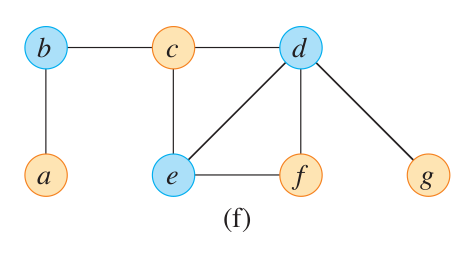
\includegraphics[width=0.3\textwidth]{figs/chap08/1108-vertex-cover-res}
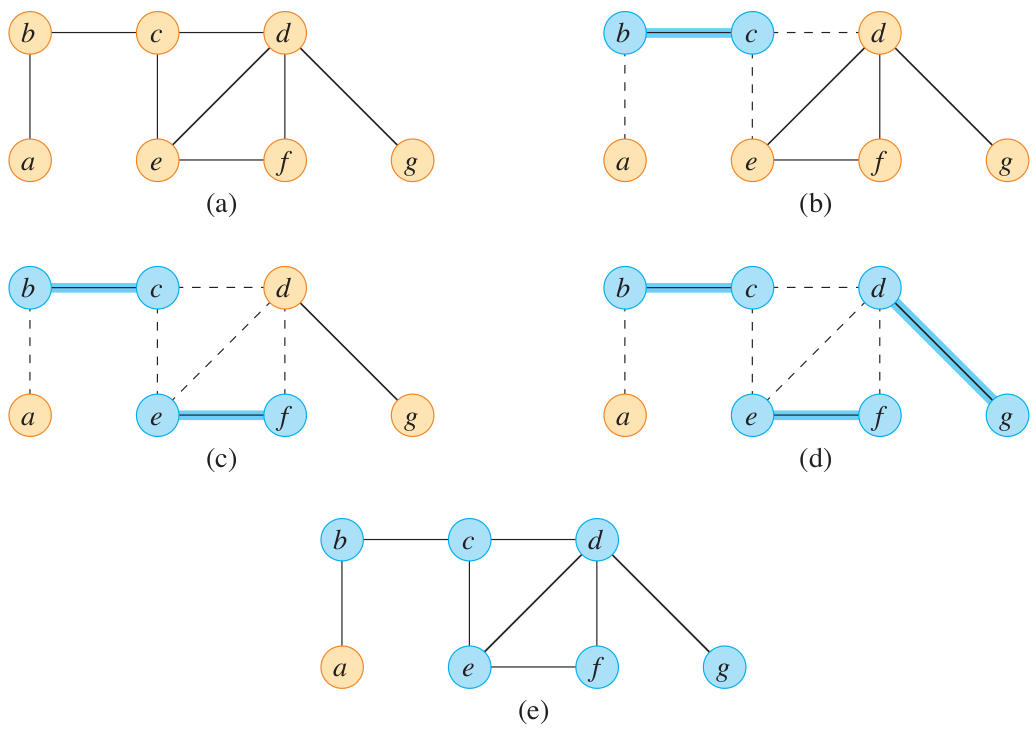
\includegraphics[width=0.6\textwidth]{figs/chap08/1108-vertex-cover}
\end{figure}
\end{itemize}
\end{frame}


\begin{frame}{‌مسئلهٔ پوشش رأسی}
\begin{itemize}\itemr
\item[-]
قضیه : الگوریتم تقریبی پوشش رأسی یک الگوریتم چند جمله‌ای تقریبی با ضریت ۲ است.
\item[-]
اثبات : مجموعهٔ
\m{C}
یک پوشش رأسی است زیرا الگوریتم در حلقه تا وقتی تکرار می‌شود که همهٔ یال‌های
\m{G.E}
با یکی از رئوس
\m{C}
پوشش داده شده‌اند.
\item[-]
حال می‌خواهیم ثابت کنیم این الگوریتم یک الگوریتم تقریبی با ضریب ۲ است.
\item[-]
فرض کنید
\m{A}
مجموعه‌ای از یال‌ها باشد که در خط ۴ الگوریتم انتخاب شده‌اند. برای اینکه یال‌های مجموعه
\m{A}
پوشش داده شوند، هر پوشش رأسی باید حداقل یکی از دو رأس هریال در
\m{A}
را شامل شود. هیچ دو یالی در
\m{A}
رأس مشترک ندارند، زیرا وقتی یک یال در خط ۴ انتخاب شد، همهٔ یال‌هایی که با آن یال رأس مشترک دارند از مجموعه
\m{E'}
در خط ۶ حذف می‌شوند.
\end{itemize}
\end{frame}


\begin{frame}{‌مسئلهٔ پوشش رأسی}
\begin{itemize}\itemr
\item[-]
بنابراین هیچ دویالی در
\m{A}
با یک رأس از
\m{C^*}
پوشش داده نشده‌اند و این بدین معنی است که به ازای هر رأس در
\m{C^*}
، حداکثر یک یال در
\m{A}
وجود دارد و بنابراین داریم :
\begin{align*}
\m{|C^*| \geqslant |A|}
\end{align*}
\item[-]
هر اجرای خط ۴ یک یال را انتخاب می‌کند که هیچ‌کدام از دو رأس مجاور آن در
\m{C}
نیستند و بنابراین داریم :
\begin{align*}
\m{|C| = 2 |A|}
\end{align*}
\item[-]
با استفاده از دو رابطهٔ به دست آمده خواهیم داشت :
\begin{align*}
\m{|C| = 2 |A| \leqslant 2|C^*|}
\end{align*}
و قضیه بدین ترتیب اثبات می‌شود.
\end{itemize}
\end{frame}

\begin{frame}{نتیجه‌گیری}
\begin{itemize}\itemr
\item[-]
یک الگوریتم روشی است گام‌به‌گام برای حل یک مسئلهٔ محاسباتی.
\item[-]
روش‌های گوناگون برای طراحی یک الگوریتم برای یک مسئله محاسباتی وجود دارد.
\item[-]
برای یک مسئله ممکن است الگوریتم‌های متفاوت با رویکردهای متفاوت وجود داشته باشد. دو معیار مهم سنجش الگوریتم‌ها زمان اجرا و میزان حافظه استفاده شده توسط آنها است. ممکن است یک الگوریتم زمان اجرای بسیار بالایی داشته باشد ولی میزان حافظهٔ مورد نیاز آن نیز بسیار بالا باشد. چنین الگوریتمی در موقعیت‌هایی کاربرد دارد که زمان اجرا مهم‌ترین معیار سنجش است.
برای مثال در سیستم‌های بلادرنگ نیاز به زمان پاسخ پایین وجود دارد.
 الگوریتم دیگری می‌تواند زمان حافظهٔ بسیار کمی استفاده کند ولی زمان اجرای آن نیز نسبتا پایین باشد چنین الگوریتمی در موقعیتی کاربرد دارد که میزان حافظه بسیار حائز اهمیت است. برای مثال در سیستم‌های نهفته حافظه محدود است. همچنین زمان اجرا و میزان حافظه مورد نیاز یک الگوریتم ممکن است حد وسط باشد. چنین الگوریتمی وقتی استفاده می‌شود که هر دو معیار زمان و حافظه به یک اندازه اهمیت داشته باشند.
\end{itemize}
\end{frame}


\begin{frame}{نتیجه‌گیری}
\begin{itemize}\itemr
\item[-]
روش‌ها و رویکردهای متفاوتی را برای حل مسائل محاسباتی از جمله روش تقسیم و حل، برنامه‌ریزی پویا، حریصانه و جستجوی فضای حالت را بررسی کردیم.
\item[-]
روش‌های تقسیم و حل و برنامه‌ریزی پویا و حریصانه برای حل مسئله در زمان چندجمله‌ای به کار می‌روند. اما مسئله‌های زیادی وجود دارند که هنوز الگوریتم چندجمله‌ای برای آنها دریافت نشده است و بنابراین برای حل اینگونه مسائل باید همهٔ جواب‌های احتمالی بررسی شوند تا جواب مورد نظر پیدا شود.
\item[-]
چنین الگوریتم‌هایی در دستهٔ الگوریتم‌های جستجوی فضای حالت یا جستجوی ترکیبیاتی قرار می‌گیرند.
\end{itemize}
\end{frame}


\begin{frame}{نتیجه‌گیری}
\begin{itemize}\itemr
\item[-]
 اگر فضای حالت بسیار بزرگ باشد ممکن است حتی برای مسئله‌های نسبتاً کوچک رویکرد جستجوی ترکیبیاتی در زمان معقول پاسخگو نباشد.
 روش پسگرد روشی است که برای بررسی فضای حالت به طور منظم استفاده می‌شود و تعدادی از حالات حذف می‌شوند.
همچنین در مسائل بهینه‌سازی به منظور کاهش تعداد حالات از روش شاخه و کران برای کوچک‌کردن فضای حالت استفاده می‌کنیم.
\item[-]
مسائلی وجود دارند که برای آنها الگوریتم چند جمله‌ای یافته نشده است، اما الگوریتم‌های تقریبی وجود دارد که در زمان چند جمله‌ای جواب نزدیک به جواب دقیق یا به عبارت دیگر جوابی تقریبی برای مسئله پیدا می‌کنند. در الگوریتم‌های تقریبی اثبات می‌شود جواب تقریبی یافته شده توسط الگوریتم چه میزان انحراف از جواب دقیق مسئله خواهد داشت.
\end{itemize}
\end{frame}
%%%%%%%%%%%%

%%%%%%%%%%%%
%\section*{References}
%\begin{frame}<0>[noframenumbering]
%\bibliographystyle{apalike}
%\bibliography{docs/bib}
%\end{frame}
%%%%%%%%%%%%

\end{document}
